\documentclass[12pt, twoside]{article}
\usepackage{setspace}

\usepackage{amsmath, amssymb, amscd, amsthm, amsfonts}
\usepackage{graphicx}
\usepackage{hyperref}
\usepackage{acronym}
\usepackage{listings}
\usepackage[a4paper, inner=4cm, outer=2.5cm, top=2cm, bottom=2cm]{geometry}
\usepackage{endnotes}
\usepackage{subfigure}
\usepackage{wrapfig}
\usepackage{mathtools}
\usepackage{blindtext}
\usepackage{fancyhdr}
\usepackage[nottoc]{tocbibind}
\usepackage{tikz}
\usepackage{multirow}

% change language to german
\usepackage[scaled=0.9]{helvet}
\usepackage{courier}
\usepackage[utf8]{inputenc}
\usepackage[T1]{fontenc}
\usepackage[ngerman]{babel}
\usepackage{hyphenat}
\usepackage{microtype}
% ---------

% for titleing
\usepackage{titling}

\newcommand{\subtitle}[1]{%
  \posttitle{%
    \par\end{center}
    \begin{center}\large#1\end{center}
    \vskip0.5em}%
}
% -----------

\begin{document}

\pagenumbering{gobble}

\tableofcontents
\pagebreak
\pagenumbering{roman}
\listoffigures
\pagebreak
\listoftables
\pagebreak

\section*{Abkürzungsverzeichnis}
\addcontentsline{toc}{section}{Abkürzungsverzeichnis}
\begin{acronym}
    \acro{gui}[GUI]{Graphical User Interface}
    \acro{eca}[ECA]{Ear-Clipping-Algorithmus}
    \acro{dt}[DT]{Delaunay Triangulation}
    \acro{cdt}[CDT]{Constrained Delaunay Triangulation}
    \acro{tm}[TM]{Turingmaschine}
    \acro{cpu}[CPU]{Central Processing Unit}
    \acro{fist}[FIST]{fast industrial-strength triangulation framework}
    \acro{sp}[SP]{Steiner Punkte}
    
\end{acronym}
\pagebreak

\pagenumbering{arabic}

\begin{onehalfspacing}

\section{Einleitung}

Die größte technische Wende nach der industriellen Revolution war die digitale Revolution gegen Ende des 20. Jahrhunderts.\cite{digrev}
Eingeleitet durch die Entwicklung des Mikrochips und der damit verbunden Verbreitung des Computers in allen Lebensbereichen führte sie 
zu einer dramatischen Veränderung. Nicht nur in der Industire und Produktion fanden diese tiefgreifenden Umbrüche statt, welche sich in flexibler Automatisierung äußerten,
sondern auch in anderen Bereichen. So wurde die Entwicklung des Internets durch vernetzte Rechner möglich.
Als dann Computer nicht mehr nur in der Forschung und für die automatische Produktion genutzt wurden, sondern auch für den täglichen Gebrauch im Büro und 
daheim etablierten, benötigte man grafische Benutzeroberflächen und Betriebssysteme. Doch dort machte die Entwicklung nicht halt.
Auch die Unterhaltungsbranche erfuhr mit Videospielen eine Revolution, welche ebenso auf Computergrafik angewiesen ist wie ein einfaches \ac{gui}.

Zu Beginn beschränkte sich die Darstellung auf sogenannte ASCII-Art, bei der übliche Zeichen aus dem ASCII-Alphabet benutzt wurden, um komplexe Bilder zu erzeugen.
Da dies jedoch nicht genügte, um Flächen und Objekte lückenlos darzustellen, bedurfte es einer Innovation. Obwohl es für Menschen einfach ist, Flächen als Ganzes zu betrachten und
Polygone in unterschiedlichster Komplexität zeichnerisch darzustellen, ist es für Computer nicht so einfach, diese zu speichern, geschweige denn darzustellen.
Flächen und dreidimensionale Objekte kann man, so die Idee, über ihre Eckpunkte (Vertices) und die dazwischen liegenden Kanten (Edges) zu repräsentieren. 
Man erzeugt also ein Polygonnetz, welches den Körper abbildet. Dabei ist die Wahl des Polygons zunächst irrelevant. So könnte man 
beispielsweise einen Würfel, abhängig von der Definition der Kanten, aus Quadraten oder Dreiecken aufbauen.\cite{polynet}
In der Praxis sind Polytope und Polygone jedoch meistens unregelmäßig, ergeben sie sich doch zum Beispiel aus Umgebenungsscans mit einem Laser-Scanner oder der Oberfläche einer Videospielfigur.
Es bietet sich in solchen Fällen nicht an, regelmäßige Polygone, wie Quadrate oder Rechtecke, als Grundlage für das Polygonnetz zu nutzen.

Eine geeignete Methode, um diese komplexen Polygone für Computer effizient darzustellen, ist die Nutzung von Dreiecken als primitive Form für die Zerlegung.
Dieses Vorgehen bezeichnet man als Triangulation. Diese ist formal die Zerlegung eines topologischen Raumes, hier also eines Polygons, in Simplexe. Das Simplex der zweiten Dimension das Dreieck und damit ist die Triangulation
ein Verfahren zur Zerlegung eines Poylgons in Dreiecke.
Es sei erwähnt, dass es Computern durchaus möglich ist, Flächen und Körper darzustellen, welche nicht aus Dreiecken bestehen. Dies ist jedoch wesentlich speicher- und rechenaufwendiger, als es bei
Dreiecken der Fall ist. Für die Darstellung eines Objektes ließe sich alternativ auch eine sogenannte Punktwolke nutzen. Wie der Name bereits andeutet, wird das Objekt dabei aus einer großen Menge
von Einzelpunkten gebildet. Für einen hohen Detailgrad sind dafür allerdings auch sehr viele Punkte nötig, was den Speicheraufwand stark erhöht. Bei der Verwendung von Dreiecken handelt es sich, vorallem
bei runden Objekte, eher um eine Approximation der Form. Eine Kugel wäre dann nicht vollständig rund, sondern würde als Polyeder repräsentiert werden. Dadurch spart man jedoch sehr viel Speicherplatz.
Man kann auch hier den Detailgrad steigern, indem man die Anzahl der Dreiecke erhöht und ihre Größe reduziert. Da Dreiecke Flächen sind, benötigt man von ihnen jedoch eine geringere Anzahl, um ein Objekt darzustellen, als wenn dies mittels einer Punktwolke geschieht.

Um eine Triangulation per Computer durchzuführen, bedarf es eines Algorithmus, der das Verfahren beschreibt. Von diesen gibt es viele verschiedene, welche unterschiedlichste Herangehensweisen nutzen.
Hier seien der Ear-Clipping-Algorithmus (\ac{eca}) und die monotone Triangulation als Beispiel für Algorithmen genannt. Des weiteren sollen hier die \ac{dt} als Triangulation mit besonderen Eigenschaften und das Voronoi-Diagramm als duale Form zur \ac{dt} angeführt werden. 
Diese unterscheiden sich erheblich in ihrer Komplexität und Effizienz. 
Mit einer Laufzeit von $O(n^2)$\cite{earclipping2}, ist der \ac{eca} bei weitem nicht so effizient wie beispielsweise ein Algorithmus zur Erzeugung einer \ac{dt} mit $O(n\log n)$. Für den \ac{eca} spricht jedoch seine relative Einfachheit im Vergleich zu anderen Algorithmen.\linebreak 

In dieser Arbeit soll jedoch nicht die Laufzeitoptimierung im Vordergrund stehen, sondern die Anschaulichkeit. Sie ist ein wichtiger Punkt, wenn es um Didaktik geht.
Anschauliche Lehrmaterialen förderen das Verständnis und bieten Interaktivität. So hat diese Ausarbeitung zum Ziel, eine interaktive Visualisierung für die Triangulation von Polygonen zu schaffen.
Dafür ist der \ac{eca} aufgrund seiner relativen Einfachheit gut geeignet. Er lässt sich schrittweise durchlaufen und ist somit sehr anschaulich, da in jedem Schritt ein 
Dreieck der Triangulierung erzeugt wird. Es liegt in der Natur dieses Algorithmus, dass Uneindeutigkeiten auftreten, was die Auswahl des nächsten Dreiecks angeht. Diese 
führen zum zweiten wichtigen Punkt in dieser Arbeit - der Interaktivität. Der Nutzer der Visualisierungssoftware soll interaktiv entscheiden können, welches das nächste 
Dreieck ist, welches bearbeitet wird. Er beeinflusst somit direkt das endgülige Resultat. Neben dem dirketen Eingriff des Nutzers sollen auch Heuristiken zu Einsatz kommen, 
um diese Auswahl zu treffen. Beispielsweise kann hierfür die Größe des Dreiecks im Bezug auf seinen Flächeninhalt genutzt werden oder auch die Innenwinkel. 
Es ist angestrebt, dass die Nutzerauswahlen ausgewertet und in eine Heuristik überführt werden. Um dies zu bewerkstelligen, soll die Qualität der Triangulation mittels verschiedener 
Metriken beurteilt werden. Hierfür kann ein Vergleich zum Voronoi-Diagramm ebenso wie zum Beispiel die Anzahl der sogenannten \emph{Slivers}\cite{sliver} betrachtet werden. 
Letztere führen in Anwendungen der Computergrafik oft zu Fehlern, welche vermieden werden sollten.

Es soll somit nicht nur eine Visualisierung für Triangulationen geschaffen werden, sondern es sollen auch die Auswirkungen einfahcer Heuristiken auf die Qualität 
dieser Zerlegungen betrachtet werden. Es steht dabei, wie bereits erwähnt, nicht die Laufzeit des Algorithmus im Vordergrund, welche üblicherweise Ziel der Optimierung ist.


\section{Theoretische Grundlagen}

\subsection{Polygone}
\subsubsection{Definition}

Ein geschlossener  Streckenzug, also eine Folge von Strecken, welche jeweils einen Endpunkt mit ihrem Vorgänger bzw. Nachfolger gemeinsam haben bilden ein \textbf{Polygon}.

\begin{wrapfigure}{hr}{0.25\textwidth}
  \centering
  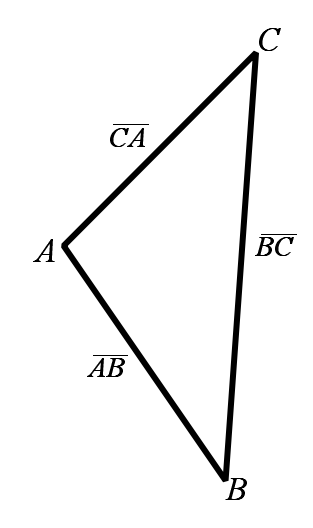
\includegraphics[width=0.2\textwidth]{bilder/dreieck_abc.png}
  \caption[Ein Dreieck als Beispiel für ein Polygon]{\centering Dreick mit Ecken $A, B, C$ als Beispiel für ein Polygon}
  \label{fig:triangle}
\end{wrapfigure}

Dabei ist es wichtig, dass die Anzahl von Strecken endlich ist. "Das Polygon, [zu Deutsch Vieleck], ist also eine durch eine Folge von Strecken begrenzte ebene Fläche." \cite{polydef}
Das einfachste Beispiel hierfür ist ein Dreicke. Es besitzt die Eckpunkte $A$, $B$ und $C$ und wir daher vom Streckenzug aus den Strecken $\overline{AB}$, $\overline{BC}$, $\overline{CA}$ begrenzt (s. Abbildung \ref{fig:triangle}).
Mit genau diesem Prinzip lassen sich beliebig komplexe Polygone erzeugen und beschreiben. Die Strecken werden auch als \textbf{Seiten} und die Endpunkte dieser Strecken 
als \textbf{Ecken} bezeichnet. 
Es sei angemerkt, dass Kreise, obwohl sie ebenfalls ebene Flächen sind, keine Polygone sind. Das folgt daraus, dass Kreise weder Ecken noch eine Begrenzung aus Strecken besitzen.

\subsubsection{Klassifikation von Polygonen}

Es ist denkbar, dass sich die Seiten des Polygons schneiden oder berühren. Man bezeichnet dieses Polygon als überschlagen.\cite{polydef}
Des weiteren kann man Polygone in regulär und nicht regulär unterteilen.
Ein Polygon mit den $n$ Seiten $a,b,c, \ldots$  und den Innenwinkeln $\alpha ,\beta ,\gamma ,\ldots$ heißt regulär, wenn

\begin{center}
  $a=b=c=\dots$ und  $\alpha =\beta =\gamma =\dotsb$
\end{center}
gilt. In einem regelmäßigen Polygon sind demnach alle Seiten zueinander kongruent und alle Winkel gleich groß. \cite{regpoly}

Eine weitere Unterteilungsmöglichkeit lautet wie folgt.
Ein Polygon heißt \textbf{konvex}, wenn für alle Innenwinkel $\alpha _i~(i \in \mathbb{N})$ gilt:
  $\alpha _i < 180^\circ$ 
Anderenfalls heißt es \textbf{konkav}. \cite{convex}

\begin{figure}[t]
  \centering
  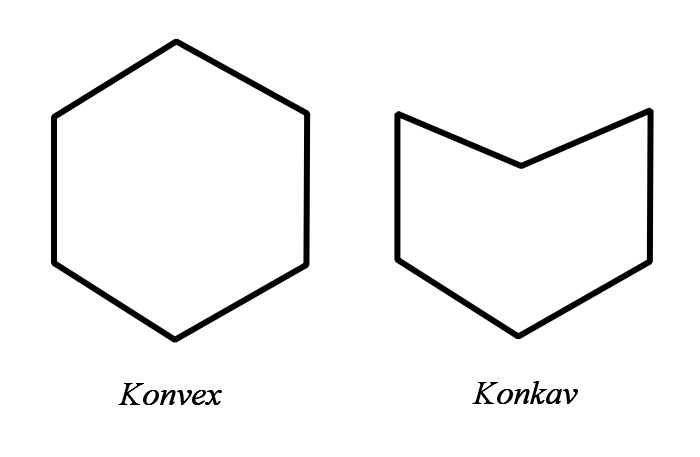
\includegraphics[width=0.5\textwidth]{bilder/konvex_konkav.png}
  \caption[Zwei Secksecke als Beispiel für konvexe bzw. konkave Polygone]{Zwei Secksecke: links konvex, rechts konkav}
  \label{fig:konvexkonkav}
\end{figure}
\pagebreak 
\subsubsection{Diagonalen}

Außer des Streckenzuges, welcher die äußere Grenze des Polygons bildet, kann man im Polygon selbst auch weitere Strecken definieren, 
welche dann als \textbf{Diagonalen} bezeichnet werden. Mittels dieser Diagonalen ist es möglich, jedes Polygon in Dreiecke zu zerlegen. 
Das wird in den nächsten Kapiteln noch näher erläutert, da dieser Sachverhalt die Grundlage für sämtliche Zerlegungsalgorithmen darstellt. 

\subsubsection{Ear und Ear Tips}

Für den in Kapitel 3.3 beschreibenen \ac{eca} ist es der Begriff des \textbf{Ear} (Ohr) relevant. 
Ein Dreieck, welches aus drei aufeinanderfolgenden Ecken $v_{i_0}, v_{i_1}, v_{i_2}$ des Polygons gebildet wird, ohne dass andere Ecken innerhalb 
dieses Dreiecks liegen oder dass der äußere Streckenzug des Polygons durch die Seiten des Dreiecks geschnitten wird, nennt man Ear. Dabei soll die 
Strecke $\left\{v_{i_0}, v_{i_2}\right\}$ eine Diagonale des Polygons. Die Ecke $v_{i_1}$ heißt dann \textbf{Ear Tip}.\cite{meister}

\begin{figure}[h]
  \centering
  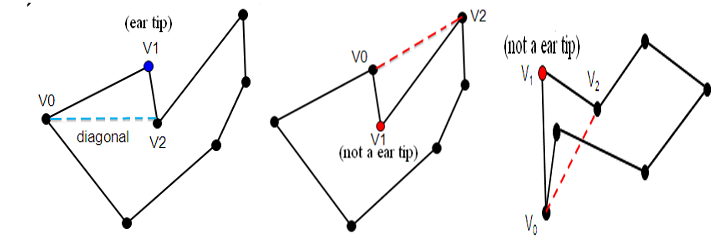
\includegraphics[width=1\textwidth]{bilder/eartips.PNG}
  \caption[Beispiele für Ear und Ear Tips in Polygonen]{\centering Links ist  $\triangle v_{i_0}, v_{i_1}, v_{i_2}$ Ear und $v_{i_1}$ Ear Tip. In der Mitte und rechts 
  ist $\triangle v_{i_0}, v_{i_1}, v_{i_2}$ kein Ear, da $\left\{v_{i_0}, v_{i_2}\right\}$ keine Diagonale ist. \cite{newAlg}}
  \label{fig:ear_eartip}
\end{figure}

\subsubsection{Sätze über Polygone}

Für Polygone gibt es einige Erkenntnisse, welche für die allgemeine Strukturanalyse von eben diesen oder auch für die Triangulation mittels 
\ac{eca} von Bedeutung sind. \break

\begin{flushleft}
  { \textbf{Satz 1 (Jordan'scher Kurvensatz):}

In der euklidischen Ebene $\mathbb{R}^2$ zerlegt jede geschlossene Jordan-Kurve $C \subset \mathbb{R}^2 $ deren Komplement $\mathbb{R}^2 \setminus C$ 
in zwei disjunkte Gebiete, deren gemeinsamer Rand die Jordankurve $C$ ist und deren Vereinigung zusammen mit die ganze Ebene $\mathbb{R}^2$ ausmacht.
\linebreak Genau eines der beiden Gebiete, das sogenannte \textbf{Innengebiet}, ist eine beschränkte Teilmenge von $\mathbb{R}^2$.
\linebreak Das andere dieser beiden Gebiete ist das sogenannte \textbf{Außengebiet} und unbeschränkt. \cite{jordan}
}
\end{flushleft}

\begin{flushleft}
{ \textbf{Satz 2 (Dreieckszerlegung:)}
  
  Jedes Polygon $P$ mit $n$ Ecken kann mittels hinzunahme von null oder mehr Diagonalen vollständig in Dreiecke zerlegt werden. \cite{newAlg}}
\end{flushleft}

\begin{flushleft}
  { \textbf{Satz 3 (Anzahl der Diagonalen:)}
  
  Jede Triangulation eines Polygons $P$ mit $n$ Ecken besteht nutzt $(n-3)$ Diagonalen und besteht aus $(n-2)$ Dreiecken. \cite{newAlg}
}
\end{flushleft}

\begin{flushleft}
  \textbf{Satz 4 (Two Ears Theorem:)}
  
  Jedes Polygon $P$ mit $n \geq 4$ Ecken besitzt mindestens zwei nicht überlappende Ears. \cite{twoears}
\end{flushleft}

\subsubsection{Polytope}
Zuletzt sei an dieser Stelle angemerkt, dass ein Polygon die zweidimensionale Ausprägung des topologischen Begriffs des \textbf{Polytops} ist.
Betrachtet man die räumlichen Dimensionen null bis vier in aufsteigender Reihenfolge so sind ein Punkt, eine Strecke, ein Quadrat, ein Würfel und ein Tesserakt.
Dies ist in der nachstehenden Abbildung zu sehen.

\begin{figure}[h]
  \centering
  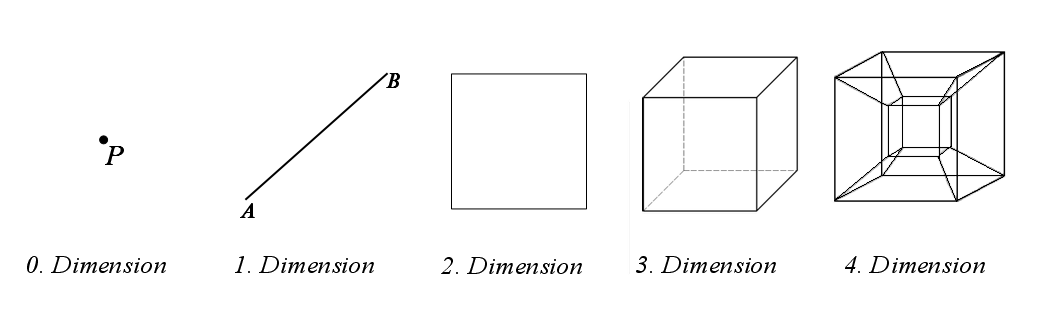
\includegraphics[width=0.9\textwidth]{bilder/Polytope_Dim0_4.png}
  \caption[Beispiele für Polytope der Dimensionen 0 bis 4]{Beispiele für Polytope der Dimensionen 0 bis 4}
  \label{fig:polytope}
\end{figure}

\subsection{Simplexe und Triangulation}

Wie bereits angesprochen kann man durch hinzufügen von Diagonalen in einem Polygon, dieses in Dreiecke oder allgemeiner in Unterpolygone 
zerlegen. Diese Eigenschaft macht sich die \textbf{Triangulation} zu nutze. Allgemein beschreibt der Begriff Triangulation die Zerlegung eines 
topologischen Raumes in \textbf{Simplexe}.\cite{polytri3} Der topologische Raum ist in diesem Fall das Polygon, welches durch einen Streckenzug gebildet wird.

Als Simplex bezeichnet man das einfachste Polygon einer Dimension.\cite{simplex} Für die nullte Dimension ist das trivialer Weise der Punkt. Da keine räumliche Ausdehnung 
möglich ist, ist der begrenzende Streckenzug hier nur der Punkt selbst.
In der ersten Dimension, in welcher Objekte eine Länge aber keine Breite besitzen, ist der Streckenzug eine einzelne Strecke. Diese ist somit auch das Simplex dieser Dimension.
Für die zweite Dimension ist nun das Dreieck das Simplex. Es ist die Fläche, welche aus den wenigsten Punkten, verbunden duch Strecken, erzeugt werden kann und daher das einfachste Polygon dieser 
Dimension. 

Wie bereits beschrieben, kann jedes komplexere Polygon so durch Diagonalen zerlegt werden, dass es volständig von Dreiecken repräsentiert wird. Das ist besonders günstig für 
eine Bearbeitung durch Computer, da ein Dreieck immer eindeutig durch seine drei Eckpunkte beschrieben wird. Diese Form ist daher speichereffizienter als beispielsweise ein allgemeines Viereck, 
für welches nicht nur die Ecken, sondern auch die Kanten gespeichert werden müssten, da mehr als eine Möglichkeit existiert diese vier Punkte zu einem Streckenzug zu verbinden.

Da in der Praxis nicht nur zweidimensionale sondern auch dreidimensionale Objekte eine Rolle spielen, stellt sich die folgende Frage. Kann man diese 3D-Objekte nicht auch in ebenfalls dreidimensionale 
Simplexe zerlegen? 

\begin{wrapfigure}{l}{0.25\textwidth}
  \centering
  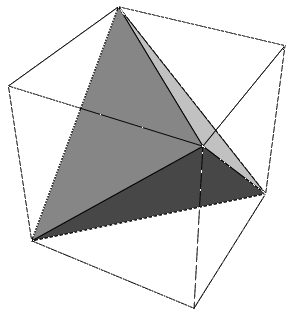
\includegraphics[width=0.2\textwidth]{bilder/cube.png}
  \caption[Zerlegung eines Würfels in vier Tetraeder]{\centering Zerlegung eines Würfels in vier Tetraeder \cite{cubecut}}
  \label{fig:cubecut}
\end{wrapfigure}

Die Antwort ist ja, jedoch ist das nicht sonderlich nützlich. Natürlich existiert in der dritten Dimension auch ein Simplex. Dieses ist der Tetraeder. Man kann auch jedes Polytop 
dieser Dimension in Tetraeder zerlegen, nur benötigt man diese Zerlegung nicht. 
Wöllte man das Innere eines Objektes durch die Zerlegung ebenfalls erhalten, beispielsweise einen Vollwürfel aus Holz in der 
Realität zersägen, dann wäre eine Tetraederzerlegung notwendig. Ein Beispiel für diese Art der Zerlegung ist in Abbildung \ref{fig:cubecut} zu sehen. 
Da man in der digitalen Welt keine echten ausgefüllten Volumina betrachtet sondern nur die Oberfläche darstellt, ist dieses verfahren für die 
Computergrafik uninteressanrt. Man kann die räumlich orientierte Oberfläche eines Würfels topologisch isomorph zu einem Würfelgitter aus quadratischen Flächen beschrieben. Diese Gesamtfläche lässt sich dann 
wiederum in Dreiecke zerlegen. Somit lässt sich auch die Oberfläche dreidimensionaler Objekte durch eine Triangulierung beschreiben. Das ist besonders gut geeigent für Computer, da man nur einen einzigen 
Algorithmus zur Bearbeitung von Flächen und Körpern benötigt, wenn man diese in Dreiecke zerlegen möchte.

\begin{figure}[h]
  \centering
  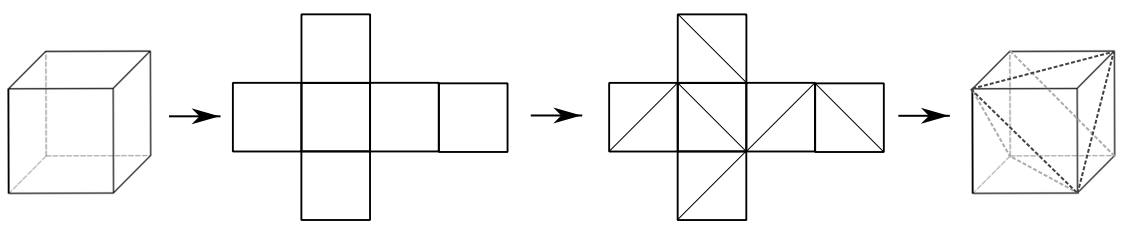
\includegraphics[width=0.9\textwidth]{bilder/3DZerlegung.png}
  \caption[Zerlegung der Oberfläche eines Würfels in Dreiecke mittels Würfelgitter]{\centering Zerlegung der Oberfläche eines Würfels in Dreiecke mittels Würfelgitter}
  \label{fig:cubenet}
\end{figure}

\subsection{Slivers}

Bei Triangulationsalgorithmen wie dem \ac{eca} liegt der Fokus zunächst nicht in der Qualität der Zerlegung. Natürlich gibt es verbesserte Versionen wie beispielsweise in Kapitel 3.1 beschreiben wird.
In jedem Fall sind sogenannte \textbf{Slivers} jedoch ein negativer Einflussfkator, wenn es um qualitative Gesichtspunkte geht. Dreiecke haben in der Computergrfaik die Eigenschaft, dass wenn man eine Scanline 
durch das Dreieck legt, dann schneidet diese ein Dreieck zweimal die Kanten des Dreieck. Diese zwei Schnittpunkte, werden von zwei unterschiedlichen Pixeln auf dem Bildschirm repräsentiert. Somit lässt sich definieren, 
wo eine Fläche beginnt und wo sie endet und dies auf dem Bildschirm darstellen. Bei Slivers ist das nicht der Fall. Ihre Innenfläche ist so schmal,
dass die beiden Schnittpunkte der Scanline mit den Kanten des Dreiecks auf den selben Pixel fallen. \cite{sliverdef} Das führt in letzter Instanz zu Grafikfehlern. 

\begin{wrapfigure}{r}{0.54\textwidth}
  \centering
  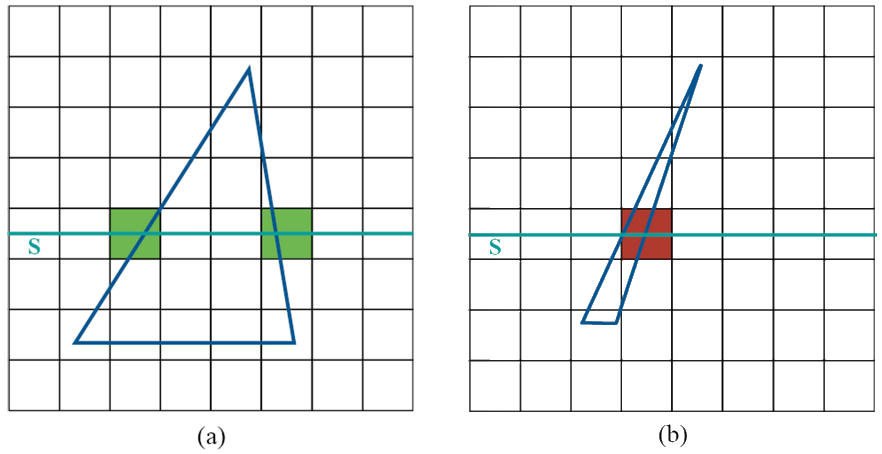
\includegraphics[width=0.49\textwidth]{bilder/sliverScanline.png}
  \caption[Unterschied Sliver und normales Dreieck]{\centering (a) Scanline mit zwei seperaten Schnittpunktpixeln (b) Sliver mit nur einem Pixel für beide Schnittpunkte}
  \label{fig:sliver}
\end{wrapfigure}

Der Begriff Sliver beschränkt sich nicht nur auf Dreiecke. Auch andere Simplexe wie Tetraeder können Simplexe sein. Dass sind diese so flach, dass auch hier Darstellungsfehler entstehen.
Zusätzlich dazu gibt es noch den verwandten Begriff der \textbf{Neadle}, der in Bezug auf Tetraeder, einen sehr schmalen aber auch sehr spitzen solchen bezeichnet.\cite{sliver} \linebreak

\subsection{Der Traditionelle Ear-Clipping-Algorithmus}

Der, in dieser Arbeit, zentrale Punkt, ist der \ac{eca}. Dieser wurde von Meister in seiner Abhandlung \emph{Polygons have ears} \cite{meister} in seiner ursprünglichen Form beschrieben.
Der Algorithmus bestimmt Dreiecke, welche die Eigenschaft eines Ears erfüllen, fügt die dafür nötige Diagonale in eine Liste ein und löscht den Punkt, welcher ein Ear Tip ist aus der Liste aller noch nicht 
bearbeiten Punkte. Dies wird solange wiederholt, bis das Restpolygon nurnoch aus drei Punkten besteht. Zuletzt wird die Lister der Diagonalen ausgegeben, da diese die Triangulation des Polygons erzeugt.
Der Algoritmus ist im Folgenden in Pseudocode dargestellt.

\begin{flushleft}
  { \textbf{Algorithmus 1: Traditionelles Ear-Clipping} \cite{improvedeca}
        \begin{tabbing}
          \=$~~~~~~$\= \textbf{Eingabe:} $~~~$\= Polyg\=on $P$ mit $n$ Ecken in einer Liste $L$\\
          \> \> \textbf{Ausgabe:} \> Liste $D$ mit $n-3$ Diagonalen, die eine Triangulierung bilden.\\
          \> \> \textbf{Schritt 1:} \>Sei $D := \emptyset$ Liste der Diagonalen.\\
          \> \> \textbf{Schritt 2:} \>\textbf{while} $|L| > 3$ \textbf{do}\\
          \> \>                     \> \> (a) Finde ein Ear $v_{i-1}, v_i, v_{i+1}$\\
          \> \>                     \> \> (b) $D := D \cup \left\{v_{i-1} v_{i+1}\right\}$\\
          \> \>                     \> \> (c) $L := L\setminus v_i$\\
          \> \> \> \textbf{endwhile}\\
          \> \> \textbf{Schritt 3:} \> Ausgabe von $D$ als triangulierende Diagonalen.
        \end{tabbing}
}
\end{flushleft}

Dieser Algoritmus hat einen Zeitaufwand von $O(n^3)$ mit einem Aufwand von $O(n^2)$ für das Ermitteln des Ear-Status eines Dreiecks. 
In dieser Formulierung wird nicht auf die Klassifikation eines Ears im speziellen eingegangen. Hierfür beginnt man klassisch 
beim ersten ersten Punkt in $L$. Man überprüft ob dieser Punkt $v_i$ konvex ist. Ist das der Fall, dann muss die Strecke $\left\{v_{i-1}v_{i+1}\right\}$ die Eigenschaft haben, 
eine Diagonale von $P$ zu sein. Wenn das ebenfalls zutrifft, dann ist das Dreicke $v_{i-1}, v_i, v_{i+1}$ ein Ear. 
Man kann die Klassifikation so darstellen:

\begin{flushleft}
  { \textbf{Algorithmus 2: Ear Klassifikation}
        \begin{tabbing}
          \=$~~~~~~$ \= \textbf{Eingabe:} $~~~$\=  Ecken \=${v_i, v_{i-1}, v_{i+1}} \in L$  $~~~~~~~~$\= \\
          \> \> \textbf{Ausgabe:} \> $\triangle v_{i-1}, v_i, v_{i+1}$ ist Ear oder nicht.\\
          \> \> \textbf{Schritt 1:} \>\textbf{if} $v_i$ konvex\\
          \> \> \> \>\textbf{if} $\left\{v_{i-1}v_{i+1}\right\}$ ist Diagonale von $P$\\
          \> \> \> \> \>Ausgabe $\triangle v_{i-1}, v_i, v_{i+1}$ ist Ear.\\
          \> \> \> \> \textbf{else} \>Ausgabe $\triangle v_{i-1}, v_i, v_{i+1}$ ist kein Ear.\\
          \> \> \> \> \textbf{endif}\\
          \> \> \> \textbf{else} Ausgabe $\triangle v_{i-1}, v_i, v_{i+1}$ ist kein Ear.\\
          \> \> \> \textbf{endif}\\
        \end{tabbing}
}
\end{flushleft}
Diese Klassifikation könnte man auch zuerst über alle Punkte $v_i$ in $L$ laufen lassen. Man spricht dann von der Klassifikationsphase. 
Danach kann man in einer zweiten Phase, der Cutting-Phase, Dreicke auswählen, welche die Ear-Eigenschaft erfüllen und sich nicht überschneiden, 
und diese dann Abschneiden. Mit diesen beiden Phasen im Wechsel kann man ebenfalls eine Triangulation erreichen. 
O'Rourke beschreibt in seinem Buch einen Ansatz, der einige Zeitersparnis bei diesem Algorithmus bewirkt.\cite{orourke}
Anstatt nach dem Abtrennen eines Ear Tip Punkts den Status jedes Eckpunktes erneut zu überprüfen, muss man nur den Status von $v_{i-1}$ und $v_{i+1}$ erneut betrachten.
Nur diese beiden Punkte sind nämlich vom Abtrennen von $v_i$ beeinflusst. Somit benötigt man insgesamt nurnoch eine Zeit von $O(n^2)$.\cite{newAlg} 
In jedem Cutting-Schritt kann man dann zusätzlich entscheiden, welche Dreieck als nächstes ausgewählt werden soll. So könnte an nur die Dreiecke auswählen, welche einer bestimmten Heuristik entsprechen.
Beispielsweise könnten so nur Dreiecke gewählt werden, bei denen der kleinste Innenwinkel das Maximum aller aktuell verfügbaren Innenwinkel ist. Auf diese Weise ist es denkbar,
dass man Sliver vermeiden könnte. Andere Ansätze sind exemplarisch im folgenden Abschnitt aufgeführt.
\section{Verwandte Arbeiten}
\subsection{Verbesserungen des Ear-Clipping-Algorithmus}

Wenn man einen Algorithmus mathematisch betrachtet, dann ist die Zeit, welcher er bis zur Terminierung benötigt, zumeist der
Gegenstand der Betrachtung. Mittels der Komplexitätstheorie lässt sich eine vom Computertyp unabhängige Beschreibung dafür finden. 
Das Referenzmodell ist dabei zumeist die \ac{tm}.\cite{tm} Ziel ist es, dass ein Algorithmus 
auf einer \ac{tm} in Polynomialzeit abläuft. Diese Zeit hängt zumeist von der Eingabegröße ab. Für den \ac{eca} ist die entscheidende 
Größe die Anzahl der Ecken $n$ des Polygons $P$.
Betrachtet man den \ac{eca} auf einer \ac{tm}, so hat er eine Komplexität von $O(n^3)$.
Zwar ist dieser Term ein Polynom in $n$, jedoch ist das kein Grund für die Wissenschaft, hier mit der Optimierung aufzuhören.
Wie O'Rourke in seiner Arbeit zeigt, kann man den \ac{eca} durch kleine Änderungen so modifizieren, dass dieser eine Komplexität von $O(n^2)$
aufweist.\cite{orourke} Diese Erkenntnis nutzen Mei, Tipper und Xu, um den Algorithmus auf andere Art zu verbessern.\cite{earclipping}

Für einen Algorithmus wie den \ac{eca} ist nicht nur seine Laufzeit entscheidend. Während andere Algorithmen beispielsweise Entscheidungsprobleme lösen, 
bei denen es nur um die Frage nahc der Existenz der Lösung geht, ist bei einer Triangulation bereits bekannt, dass es unterschiedliche Lösungen gibt.
Daher ist die Frage nicht, ob eine Lösung existiert, sondern ob eine optimale solche gefunden werden kann. Optimal ist dabei ein relativer Begriff, 
der stark von den Rahmenbedingungen abhängt. Für den \ac{eca} ist der Speicherbedarf ebenfalls entscheidend. Dieser ist bei Mei, Tipper und Xu durch $O(n)$
begenzt. Das Ziel ihrer Arbeit war es, qualitytiv hochwertige Triangulationen für komplexe Polygone zu erzeugen. Der Qualitätsparameter war dabei der kleinste 
Innenwinkel der erzeugten Dreiecke in der Zerlegung. Genauer ging es darum, die sogenannten Slivers zu vermeiden (s. Kapitel 2.3).

Ihr Ansatz war es, den verbesserten Algorithmus von O'Rourke so zu modifizieren, dass er über die Option des \textbf{Edge Swappings} verfügt.
Wird ein Ear erkannt, dann wird für jeden seiner Innenwinkel überprüft, ob dieser kleiner ist als ein zuvor festgelegter Grenzwert. Ist das der Fall, dann 
muss bei diesem Dreieck Edge Swapping durchgeführt werden. Dafür werden der größte Innenwinkel des Dreiecks und die, ihm gegenüberliedende, längste Seite bestimmt.
Daraufhin wird überprüft, ob es ein Nachbardreieck gibt, welches sich mit dem Ursprünglichen eben diese längste Seite teilt. Gibt es einen solchen Nachbarn, 
dann wird in dem von den beiden Dreiecken gebildeten Viereck eine Diagonale zwischen den beiden Ecken gezogen, welche jeweils der zuvor bestimmten längsten Seite gegenüber lagen.
Auf diese Art entstehen wieder zwei Dreiecke, von denen nun die Innenwinkel auf ihre Größe überprüft werden. Ist jeweil der kleinste Winkel größer als der Grenzwert, 
dann ist die Qualität der Dreiecke nun besser als die des ursprünglich Ausgewählten. Wenn dem nicht so ist, bleibt alles unverändert und das Ear wird wie es war gewählt und abgeschnitten.

%Grid Impementierung FIST
% Im FIST-Paper wird noch auf eine weitere wichtige Verbesserungstechnik eingegangen: Spatial-Hashing-Verfahren (z.B. Grids), um die Menge der Vertices einzuschränken, 
% die pro potentiellem Ear getestet werden. Kannst Du darauf evtl. noch eingehen? So ein Grid ist auch in meiner Rust-Implementierung enthalten.

\begin{figure}
    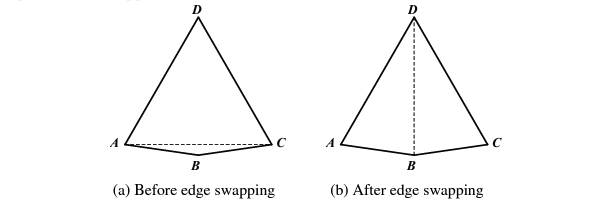
\includegraphics[width=1\textwidth]{bilder/edgeswapping.png}
    \caption[Edge Swapping]{Edge Swapping \cite{earclipping}}
    \label{fig:edgeswapping}
\end{figure}

Auf diese Art kann die Qualität der Dreiecke in der Triangulation stark erhöht werden. Sie zeigen an Beispielen, dass sich die Innenwinkelgröße durchschnittlich verdoppelt.
Teilweise können Dreiecke mit minimalem Innenwinkel von $< 15^\circ$ ganz eliminiert werden. Das hängt jedoch vom eingegebenen Poylgon ab und hat keine Allgemeingültigkeit.

\subsection{Parallelisierung des Ear-Clipping-Algorithmus}

Anstatt den Algorithmus selbst in seiner Laufzeit zu verbessern, ist es ein Gedanke, die Abarbeitung aufzuteilen. Vorallem mit der technischen Entwicklung mehrerer Prozessorkerne in einer \ac{cpu}
ist verteiltes Rechnen ein gängiges Konzept. Hierzu haben Eder, Held und Palfrader eine Arbeit verfasst, die sich mit der Umsetzung des \ac{eca} unter dem Gesichtspunkt der coarse-grain parallelization,
zu Deutsch grobkörnigen Parallelisierung, befasst.\cite{paralleleca} Dieses Prinzip beschreibt die Aufteilung eines Programms in längere Unteraufgaben. Das ist ein für Multicore Computer sehr geeignetes Konzept.
Andere Arbeiten befassten sich auch mit der Umsetzung der Arbeitsteilung, aber dort speziell mit dem Konzept der fine-grain parallelization im Bezug auf die \ac{dt}. Die fine-grain parallelization, also die feinkörnige 
Parallelisierung, beschreibt die Aufteilung eines Programms in eine Vielzahl kleinerer Aufgaben. 
Hier ist beispielsweise M. Goodrich\cite{goodrich} zu nennen.

Eder, Held und Palfrader haben ihre Arbeit auf \ac{fist} aufgebaut. Dieses Framework ist ein in C++ verfasster Code für Polygontriangulation basierend auf dem \ac{eca}.\cite{paralleleca}
Sie beschränkten sich dabei mit der Parallelisierung auf den Bereich des Algorithmus, welcher sich mit der Klassifikation und dem Clipping der Ears befasst. Dieser Teil macht etwa $80\%$ des Rechenaufwandes aus.
Um eine Aufteilung in $k$ Threads zu erreichen, welche dann auf den $k$ Kernen der \ac{cpu} abgearbeitet werden sollen, nutzen Sie drei verschiedene Ansätze und vergleichen diese miteinander und mit der nicht parallel 
laufenden Form des Algorithmus in \ac{fist}.

Ihr erster Ansatz beruht auf dem \emph{divide-and-conquer-Prinzip}. Anstatt das Polygon $P$ allerding durch Diagonalen in etwa gleich große Unterpolygone $P_k$ zu unterteilen, 
nutzen Sie $k-1$ viele senkrechte Geraden dafür. Dies ist weit weniger aufwendig in der Berechnung, da das Finden von geeigneten Diagonalen relativ rechenintensiv ist.
Sie berufen sich dabei auf einen Algorithmus von Sutherland und Hodgman \cite{dnc}. Bei dieser Form der Unterteilung enstehen sogenannte \ac{sp}, welche die Schnittpunkte der senkrechten Geraden mit 
den Strecken der äußeren Begrenzung darstellen. Dafür benötigt man eine Zeit von $O(n)$ pro Gerade $l$ und fügt im schlimmsten Fall $O(n)$ \ac{sp} ein. Diese werden als neue Eckpunkte in den Unterpolygonen eingefügt und damit vom \ac{eca} auch als Eckpunkte der Dreiecke in der Zerlegung benutzt. 
Das führt dazu, dass Dreiecke in der Gesamtzerlegung von $P$ entstehen, welche unzulässige Eckpunkte besitzen, da diese im Ursprünglichen Polygon nicht existieren. 
Dafür muss eine Bereinigung der Zerlegung durchgeführt werden, nachdem alle $k$ Threads ihre Triangulation der $P_k$ Unterpolygone geliefert haben. 
Durch den Schnitt des Poylgons mit einer senkrechten Geraden entstehen zwei \ac{sp} $s_a$ und $s_b$. Um diese wieder zu löschen, werden alle Dreiecke, welche zu einem dieser beiden Punkte inzident sind, aus der Triangulation 
gelöscht. Auf diese Weise erzeugt man ein Loch $H$ in der Zerlegung, welches wieder ein Polygon ist. Diese kann man nun durch erneute Triangulation mit validen Dreiecken füllen. \linebreak 

Einen \emph{partition-and-cut-Ansatz} zu verwenden, war die zweite Variante, um die Triangulation auf die $k$ Threads aufzuteilen. Dabei wird nicht wie bei \emph{divide-and-conquer} das gesamte Polygon $P$, sondern nur sein begrenzender Streckenzug unterteilt.
Hierfür werden \textbf{Landmarks}, also Wegpunkte, eingeführt. Dies geschieht anhand der Indizierung der $n$ Ecken. Die Eckpunkte mit den Indizes $\left\{ 0, \frac{n}{k}, \frac{2n}{k}, \dots, \frac{(k-1)n}{k} \right\}$ werden die Landmarks. Der Streckenzug zwischen je zwei dieser Markierungen wird 
jeweils einem Thread zugewiesen. Die Wegpunkte gehören dabei jeweils zu zwei benachtbarten Teilstreckenzügen gleichzeitig. Jeder Thread durchläuft dann eine Klassifikations- und eine Clippingphase, bei denen darauf geachtet wird, dass die Landmarks nicht gelöscht werden.
Ist das geschehen und alle Threads beendet, dann bleibt ein Teil des Polygons noch unbearbeitet. Dieser Teil wird bei Eder, Held und Palfrader nicht nocheinaml in Abschnitte für verschiedene Threads unterteilt sondern wird dann vom sequentiellen \ac{eca} in \ac{fist} bearbeitet.
Zwischen den Threads wird keine Synchronisation benötigt, da sowohl Klassifikation als auch Clipping völlig undabhängig von anderen Threads ablaufen und nur in ihrem jeweiligen Abschnitt Dreiecke erzeugt werden. Dabei sei angemerkt, dass das Überprpüfen der Ear-Eigenschaft nur Lesezugriff auf 
die Globale Liste aller Eckpunkte des Polygons benötigt. Der Vorgang der Aufteilung in Threads und deren bearbeitung ist in der nachstehenden Abbildung zu sehen. \linebreak
\begin{figure}[h]
    \centering
    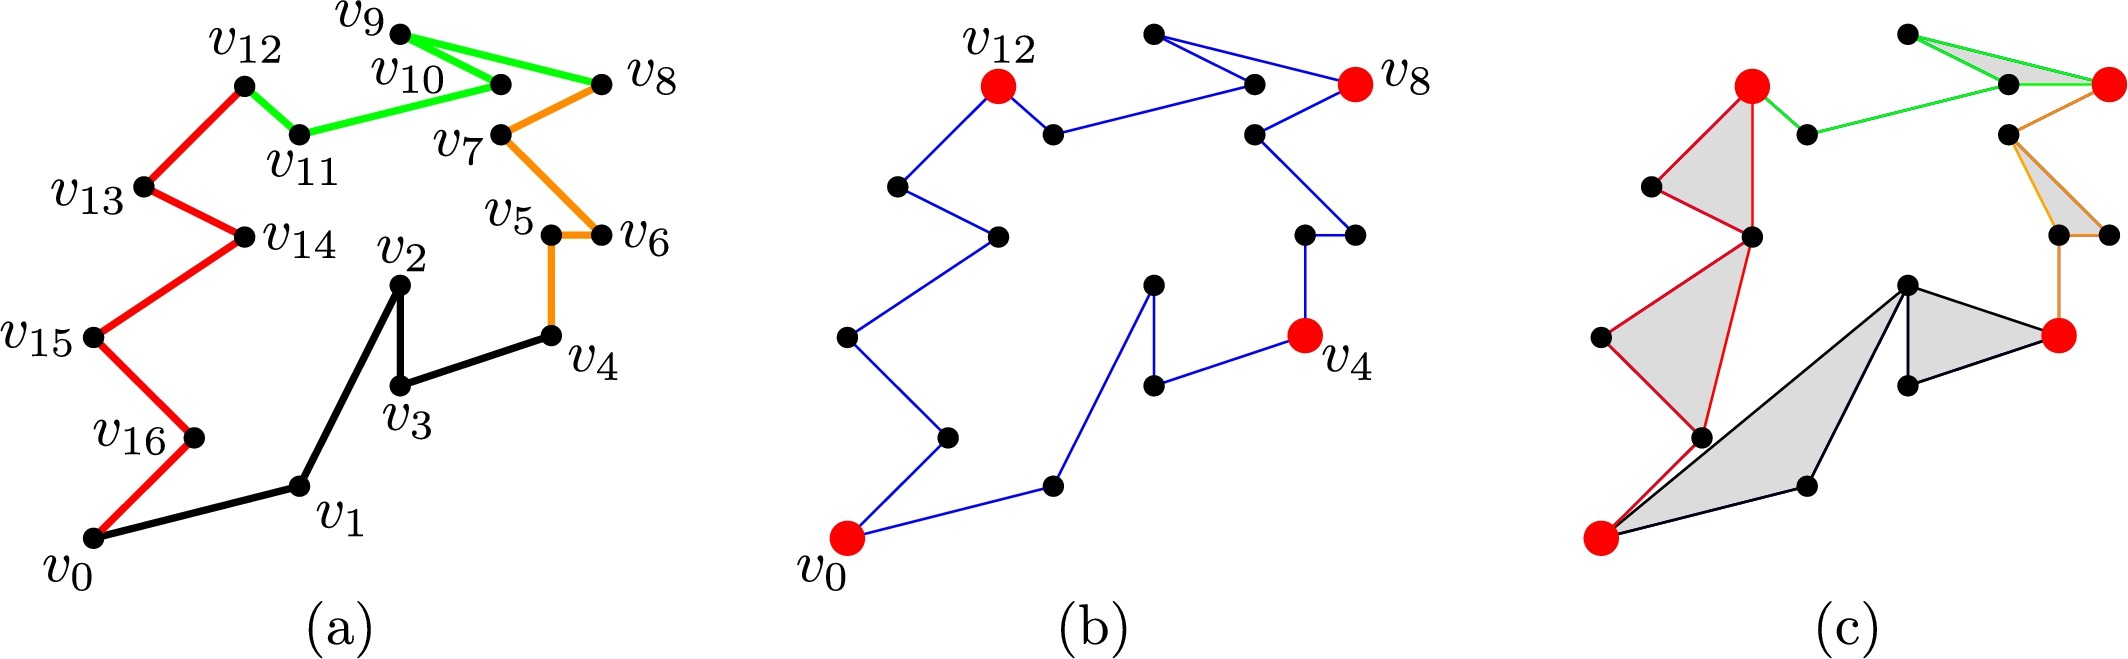
\includegraphics[width=0.8\textwidth]{bilder/segmentierung.jpg}
    \caption[Unterteilung des Streckenzugs in Unterstreckenzüge mittels Landmarks für Parallelisierung]{\centering (a) Einfaches Polygon $P$ unterteilt in vier Streckenzüge (b) Landmarks vervorgehoben (c) Triangulierung durch Threads}
    \label{fig:langmarks}
\end{figure}

Der dritte Ansatz, betreffend dem \ac{eca} in \ac{fist} ist der sogenannte \emph{mark-and-cut-Ansatz}, welcher Ähnlichkeiten zum vorher erwähnten \emph{partition-and-cut-Ansatz} aufweist. Auch in diesem Fall werden einige Eckpunkte von $P$ als Markierungen genutzt.
In der Marierungsphase, durchläuft ein Thread den Streckenzug von $P$ und speichert jeden zweiten konvexen Eckpunkt in einer Liste. Hat dieser Thread die Hälfte aller Punkte überprüft, werden die Cut-Threads gestartet, welche nur die Cutting-Phase durchlaufen. Bildet 
ein Punkt in der Liste mit seiner gegenüberliegenden Seite ein Dreiecke, dann wird dieses sofort als valide gespeichert und abgeschnitten. Jeder dieser Punkte darf nur einmal bearbeitet werden, damit es nicht zu Asynchronität und Redundanz kommt. Wenn die Cut-Threads alle ihre Arbeit getan haben, 
werden sie neu gestartet und bearbeiten dann alle Punkte, die Seit ihrem letzten Start zur Liste hinzugefügt worden sind.
Während dessen durchläuft der Mark-Thread das Polygon erneut und fürgt neue konvexe Punkte zu Liste hinzu und so weiter, bis nurnoch weniger Dreiecke erkannt werden, als vorher mit einem Grenzwert festgelegt. Dieser lag bei Eder, Held und Palfrader bei 20 Dreiecken.
Der Rest von $P$, welcher noch nicht bearbeitet wurde, wird dann wie im \emph{partition-and-cut-Ansatz} von einem sequentiellen Aufruf von \ac{fist} bearbeitet. 

\begin{figure}[b]
    \centering
    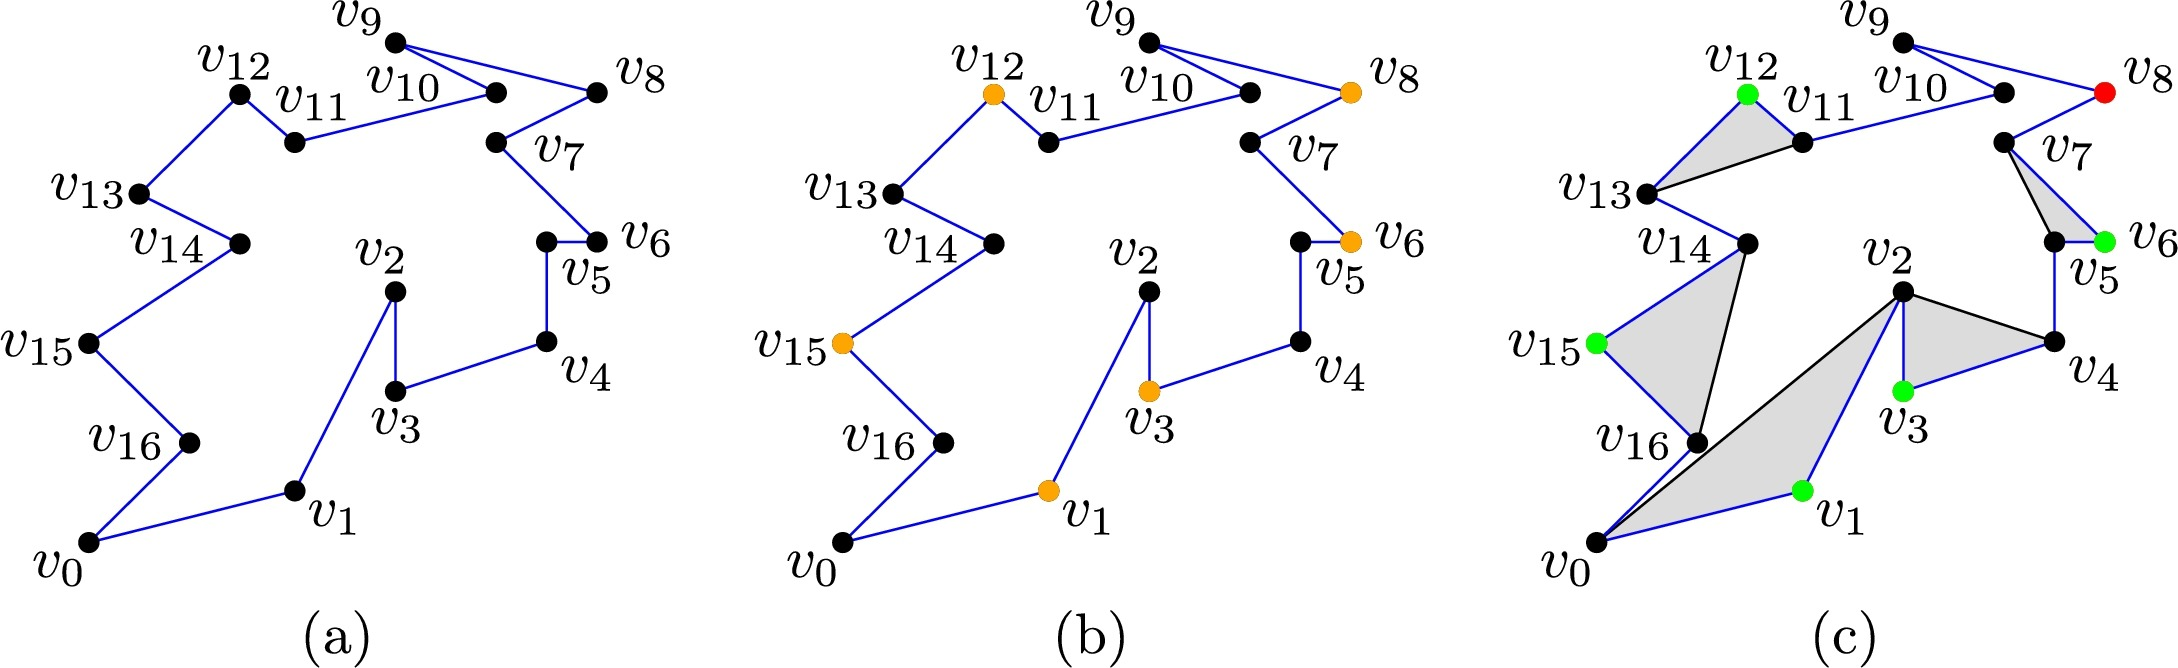
\includegraphics[width=0.8\textwidth]{bilder/markierung.jpg}
    \caption[Markierung konvexer Eckpunkte für Parallelisierung]{\centering (a) Einfaches Polygon $P$ (b) Erste Markierungsphase, ausgewählte Ecken in orange (c) Erste Cutting-Phase}
    \label{fig:konvPoints}
\end{figure}

Der finale Vergleich aller drei Ansätze hinsichtlich ihrer Qualität zeigt, dass sie in etwa gleich gut sind. Als Vergleich wurde von ihnen noch eine Variante der \ac{dt}, die sogenannte \ac{cdt} durchgeführt, auf die an dieser Stelle allerdings nicht 
genauer eingegangen werden soll. Die folgende Tabelle zeigt das Ergebnis.

\begin{table}[h]
    \begin{tabular}[h]{| l | c | c | c | c | c |}
    \hline
    & CDT & FIST's top & D\&C & P$\&$C & M$\&$C \\ \hline
    (1) Durchschn. Abw. 60° & 30.79° & 31.53° & 35.29° & 34.97° & 38.38° \\ \hline
    (2) Durchschn. min. Winkel & 24.60° & 23.40° & 20.07° & 21.32° & 21.07° \\ \hline
    \end{tabular}
    \caption[Vergleich verschiedener Parallelisierungen des \ac{eca} in \ac{fist}]{Vergleich der \ac{fist} Trianulation inklusive \ac{cdt} und FIST's top Heuristik. Aufgeführt sind folgende Parallele Versionen von \ac{fist}: 
    Divide-and-conquer D\&C, Partition-and-cut P\&C und Mark-and-Cut M\&C. 
    (1) Durchschnittliche Abweichung aller Innenwinkel von 60° über alle Triangulationen (je kleiner, desdo besser) 
    (2) Durchschnittliche Größe des kleinsten Innenwinkels aller Dreiecke über alle Trinagulationen (je größer, desdo besser) \cite{paralleleca}}
    \label{tab:tab1}
\end{table}

\subsection{Alternative Verfahren und Ansätze} 

\subsubsection{Delauny Triangulation}

Spricht man von Triangulationen, so stößt man zwangsläufig auf den Begriff der Delauny Triangulation. Sie ist, qualitativ gesehen, die Triangulation mit den ausgewogensten Dreiecken.

\begin{wrapfigure}{lh}{0.25\textwidth}
    \centering
    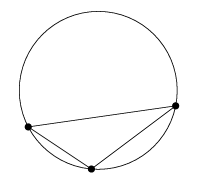
\includegraphics[width=0.23\textwidth]{bilder/umkreis.png}
    \caption[Umkreis eines Dreiecks]{\centering Umkreis eines Dreiecks \cite{delauny}}
    \label{fig:umkreis}
  \end{wrapfigure}

Um jedoch zu verstehen wie die \ac{dt} gebildet wird, benötigt man den Begriff des \emph{leeren Umkreises}. Sie ist die grundlegende Bedingung für eine \ac{dt}, da man nur solche Triangulationen, in denen alle Dreiecke eben diese 
Bedingung des leeren Umkreises erfüllen, eine \ac{dt} nennt.\cite{delauny}

Man betrachte eine Menge aus Punkten $V$ in der euklidischen Ebene $\mathbb{R}^2$. Ein Dreieck $\triangle v_1v_2v_3$ mit $v_1, v_2, v_3 \in V$ erfüllt die Bedingung des leeren Umkreises, wenn der Kreis, welcher durch die drei Punkte $v_1, v_2, v_3$ geht, 
keine anderen Punkte $v_i \in V$ beinhaltet. 

Kann man also eine Menge aus Dreiecken $T$ finden, sodass jeder Punkt der Menge $V$ teil mindestens eines Dreiecks ist und jedes Dreieck wenigstens eine Seite mit einem anderen Dreieck teilt, dann
ist die $T$ eine \ac{dt} von $V$, wenn jedes Dreieck in $T$ einen leeren Umkreis besitzt. 

Dass diese Triangulation nicht eindeutig ist, kann mann an einem einfachen Beispiel zeigen. Hat man vier Punkte im $\mathbb{R}^2$, welche alle zueinander konvex sind, dann ist es möglich, dass alle diese Punkte auf dem selben Umkreis liegen.
In einem solchen Fall sind alle möglichen Kombinationen aus sich nicht gegenseitig schneidenden Dreiecken als \ac{dt} zulässig. Jedoch gibt es auch den Fall, dass nur je drei Punkte auf einem Kreis liegen. Dafür gibt es immer zwei Möglichkeiten, von denen 
meist nur eine eine \ac{dt} ist. In Abbildung \ref{fig:fourpointdt} ist sind in den Fällen (a) und (b) diese Möglichkeiten für Umkreise zu sehen, welche einmal eine \ac{dt} erzeugen und einmal nicht. In Fall (c) ist der zuvor beschriebene Fall aufgeführt, 
bei dem die vier Punkte alle auf dem selben Kreis liegen.

\begin{figure}[h]
    \centering
    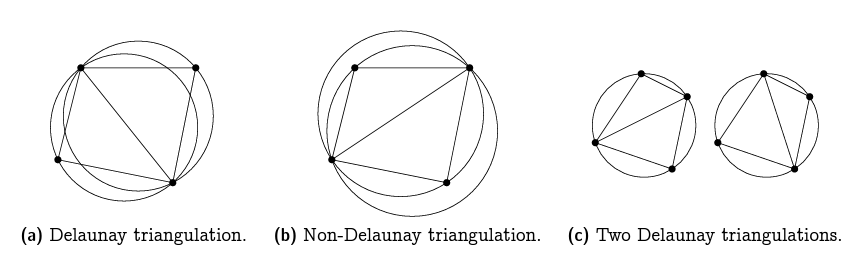
\includegraphics[width=1\textwidth]{bilder/fourpointdt.png}
    \caption[Delauny Triangulation für vier konvexe Punkte]{Delauny Triangulation für vier konvexe Punkte. (a) Delauny Triangulation (b) keine Delauny Triangulation (c) mehrere gleichwertige Triangulationen \cite{delauny}}
    \label{fig:fourpointdt}
\end{figure}

Eine sehr vorteilhafte Eigenschaft der \ac{dt}, welche diese für praktische Anwendungen sehr interessant macht, ist, dass sie den minimalen Innenwinkel jedes Dreiecks der Triangulation maximiert. Das bedeutet, dass die \ac{dt} die qualitativ hochwertigste aller möglichen Triangulationen
einer Menge von Punkten ist. Aber auch so ist es nicht möglich, dass jede \ac{dt} die Bedingung erfüllt, keine Slivers zu enthalten. Es bedeutet lediglich, dass, wenn ein Sliver teil einer \ac{dt} ist, dann wäre auch in jeder anderen Triangulation mindestens ein Sliver enthalten.
Das ist immerhin in sofern eine gute Eigenschaft, da eine \ac{dt} einer Punktmenge immer die minimale Anzahl an Slivers enthält. Sie dient damit als optimaler Vergleich für beispielsweise den \ac{eca}, da man damit die Abweichung der Triangulation des \ac{eca} zu der durch die \ac{dt} erzeugten bestimmen kann. 

\begin{wrapfigure}{hr}{0.35\textwidth}
    \centering
    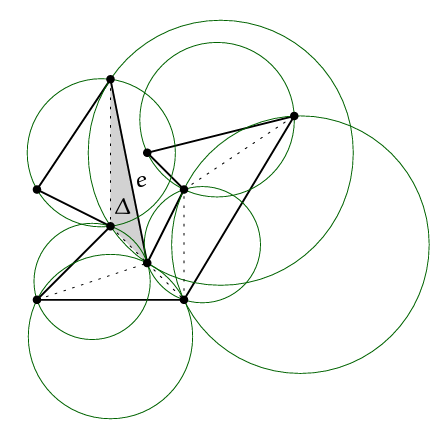
\includegraphics[width=0.35\textwidth]{bilder/cdt.png}
    \caption[Constrained Delauny Triangulation für ein Polygon]{Constrained Delauny Triangulation eines Polygons\cite{delauny}}
    \label{fig:cdt}
\end{wrapfigure}
Möchte man, wie in dieser Arbeit, ein Polygon in Dreiecke zerlegen, so stößt man auf ein Problem. Ein Polygon in zwar eine Menge aus Punkten, jedoch sind diese bereits durch einen Streckenzug fest miteinander verbunden. Man kann in dem meisten Fällen also keine echte \ac{dt} erzeugen, 
da die Dreiecke nicht frei wählbar sind. Man spricht dann von der sogenannten \ac{cdt}. Diese versucht ebenfalls die Bedingung des leeren Umkreises zu erfüllen, allerdings mit einer Einschränkung, welche sie für vorgegebene Polygone umsetzbar macht.
Der Umkreis eines Dreiecks $\triangle$ darf andere Punkte des Polygons enthalten, wenn diese von innerhalb von $\triangle$ nicht sichtbar sind. Ein Punkt $p$ heißt \textbf{sichtbar}, wenn eine Punkt $q$ im Inneren des Dreiecks $\triangle$ existiert, so dass die Strecke $\overline{pq}$ keine andere Strecke $e \in E$ schneidet.
Anderenfalls blockiert $e$ sozusagen die Sicht auf den Punkt $p$.


\subsubsection{Algorithmus basierend auf Sichtbarkeit}

Wie schon bei der \ac{dt} ist hier der Begriff der Sichtbarkeit von Eckpunkten entscheidend. Anders als zuvor werden hier jedoch keine Dreiecke ermittelt,
welche die Bedingung des leeren Umkreises erfüllen. In diesem Algorithmus, beschrieben von Ran Liu, wird das Polygon $P$ in zwei Unterpolygone $P_1$ und $P_2$ unterteilt,
welche dann solange rekursiv weiter unterteilt werden, bis die entstandenen Unterpolygone $P_i$ Dreiecke sind.\cite{newAlg}
Hierfür muss in einem ersten Schritt die Sichtbarkeit jedes Punkte gegenüber einem Referenzpunkt $v_i$ überprüft werden. Dazu betrachtet man zunächst die Nachbarn $v_{i-1}$ und $v_i+1$ 
von $v_i$. Diese begrenzen das sogenannte \textbf{Sichtfeld} von $v_i$, welches mit $\alpha$ bezeichnet wird und dem Winkel in $v_i$ entspricht. Für spätere Betrachtungen zählen $v_{i-1}$ und $v_{i+1}$ 
als nicht sichtbar im BEzug auf $v_i$. Entlang der Kanten von $P$ wird nun ausgehend von $v_{i+1}$ entgegen dem Uhrzeigersinn überprüft, ob ein Punkt $v_j$ im Sichtfeld von $v_i$ liegt.
Ist das der Fall, dann gilt der Punkt $v_j$ als sichtbar, wenn die Strecke $v_iv_j$ eine Diagonale von $P$ ist. Zusätzlich begrenzt dieser Punkt nun das Sichtfeld und es muss verkleinert werden. Das neue Sichtfeld $\alpha$ berchnet sich also durch $\alpha = v_{i-1},v_i,v_j$.
Der Vorgang wird fortgesetzt, bis alle Punkte überprüft sind. Ist diese Überprüfung für alle $v_i$ von $P$ abgeschlossen, wird die Anzahl der sichtaberen Punkte 
gegenüber dem jeweiligen Referenzpunkt bestimmt. Diese dient als Vergleichskriterum für die Punkte untereinander. Als Beispiel ist in der nachfolgenden Abbildung einmal die Ermittlung von $alpha$ und die Überprüfung 
mehrerer Punkte bezogen auf den Punkt $v_0$ dargestellt. 

\begin{figure}[h]
\centering
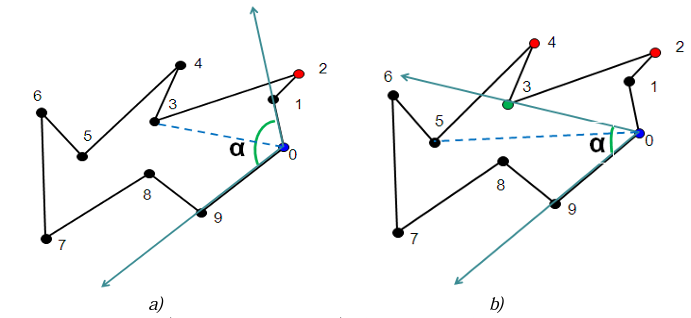
\includegraphics[width=1\textwidth]{bilder/sichtbarkeit.png}
\caption[Sichtbarkeit von Punkten]{\centering(a) $v_3$ ist sichtbar für $v_0$ (b) Überprüfung der Sichtbarkeit von $v_5$ mit neuem Sichtfeld $\alpha$ (nicht sichtbar entspricht rot, sichtbar entspricht grün) \cite{newAlg} }
\label{fig:visibPoint}
\end{figure}

Für die Anzahl sichtbarer Punkte bezogen auf $v_i$ wird die hier Bezeichnung $s(v_i)$ verwendet. Man kann diesen Vorgang der Sichtbarkeitsanalyse wie folgt in Pseudocode beschreiben.

\begin{flushleft}
    { \textbf{Algorithmus 4: Sichtbarkeitsanalyse für einen Punkt $v_i$}
          \begin{tabbing}
            \=$~~~~~~$ \= \textbf{Eingabe:} $~~~$\=  Eck\=en $v_i$\=$ \in V$\=$(P),~n = |V(P)| - 3,~s(v_i)=0$\\
            \> \> \textbf{Ausgabe:} \> Anzahl sichtbarer Punkte $s(v_i)$\\
            \> \> \textbf{Schritt 1:} \> Wähle Referenzpunkt $v_i$ \\
            \> \> \textbf{Schritt 2:} \>$\alpha = \angle v_{i-1}v_iv_{i+1}$\\
            \> \> \textbf{Schritt 3:} \>\textbf{while} $n > 0$ \textbf{do}\\
            \> \> \> \> \textbf{if} $\angle v_{i-1}v_iv_j > 0 \wedge \angle v_{i-1}v_iv_j < \alpha$\\
            \> \> \> \> \> \textbf{if} $v_iv_j$ Diagonale von $P$\\
            \> \> \> \> \> \> (a) $s(v_i)= s(v_i)+1$\\
            \> \> \> \> \> \> (b) $\alpha = \angle v_{i-1}v_iv_j$\\
            \> \> \> \> \> \> (c) $n = n-1$\\
            \> \> \textbf{Schritt 4:} \> Ausgabe von $s(v_i)$ 

          \end{tabbing}
  }
  \end{flushleft}

Ist $s(v_i)$ für jeden Eckpunkt $v_i$ von $P$ ermittelt, wird der Punkt mit der größten solchen Anzhal ausgewählt. Gibt es mehrere solche Punkte, dann 
kann ein beliebige dieser Punkte gewählt werden. Dieser Punkt wird dann als \textbf{First Head} bezeichnet.
Als nächstes wird noch der Punkt mit der zweit höchsten Anzahl $s(v_i)$ gewählt. Er wird als \textbf{Second Head} bezeichnet. Sollte es hier Uneindeutigkeiten
bei der Auswahl geben, dann wird ein Test durchgeführt, um diesen Punkt auszuwählen. Durch die Diagonale zwischen First und Second Head soll das Polygon in zwei 
Unterpolygone zerlegt werden. Man testet, bei welchem der möglichen Punkte für den Second Head, der Betrag der Differenz zwischen der Anzahl an Strecken in den beiden 
Unterpolygonen $P_1$ und $P_2$ am geringsten ist. Das ist in der nächsten Abbildung zu sehen.

\begin{figure}[h]
    \centering
    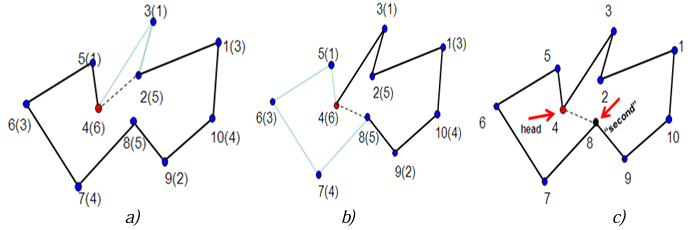
\includegraphics[width=1\textwidth]{bilder/second_head_comp.png}
    \caption[Test zur Auswahl des Second Head]{\centering(a) und (b) Vergleich der Differenz zwischen der Länge des schwazen und des türkiesen Strecknabschnitts (c) Auswahl des Second Head \cite{newAlg} }
    \label{fig:secHead}
\end{figure}

Für die Zerlegung werden First und Second Head dann dupliziert, damit beide Polygone vollständig begrenzt sind. In beiden Unterpolygonen muss dann die Sichtbarkeitsanalyse erneut durchgeführt werden.
Damit dies ein wenig schneller geschieht, kann man die sichtbaren Punkte im Bezug auf einen Punkt $v_i$ in einer sogennanten \emph{single circular list} gespeichert werden. In einer solchen Liste zeigt der Pointer des 
letzten Elements auf das erste Element der Liste. Beim Update der Sichtbarkeiten müssen dann für jeden Punkt nur die Punkte in seiner jeweiligen Liste überprüft werden und jetzt nicht mehr sichtbare Punkte aus der Liste 
gelöscht werden. Damit wird die Laufzeit der Sichtbarkeitsanalyse von $O(n^2)$ auf $O(n)$ begrenzt. Nichtsdesdotrotz hat der neue Algorithmus von Ran Liu, nach seiner eigenen groben Analyse, eine Komplexität von über $O(n^3)$.
Im Vergleich mit dem \ac{eca}, welcher eine Komplexität von $O(n^2)$ besitzt, schneidet er damit schlechter ab. In Tabelle \ref{tab:tab2} und \ref{tab:tab3} werden zwei Beispiele des Vergleichs zwischen dem Sichtbarkeitsalgorithmus 
und dem \ac{eca} aus der Arbeit von Liu angeführt. Die Algorithmen wurden auf zufällig generierten Polygone unterschiedlicher Knotenanzahl und Form getestet. Dabei waren die getesteten Polygonformen einmal \emph{rund}, das heißt 
die Eckpunkte konnten nur in einem quadratischen Koordinatenbereich liegen. Der andere Typ war \emph{länglich}, wobei die Punkte eher in ihrer x-Koordinate weiter streuten, nicht so sehr jedoch in der y-Koordinate.
Es ist in den Ergebnissen dieser Tests ersichtlich, dass die Qualität der Dreiecke bezogen auf ihre minimalen Innenwinkel bei Liu's Algorithmus besser ist, als die des \ac{eca}. In Sachen Laufzeit jedoch schneitet der neue Algorithmus jedoch schlechter ab,
wie bereits die Komplexitätsanalyse zeigte.

In der nachfolgenden Abbildung ist zunächst einmal exemplarisch dargestellt, wie eine solche Zerlegung eines einfachen Polygons durchgeführt wird.
Danach folgen die angesprochenen Tabellen.
\begin{figure}[h]
    \centering
    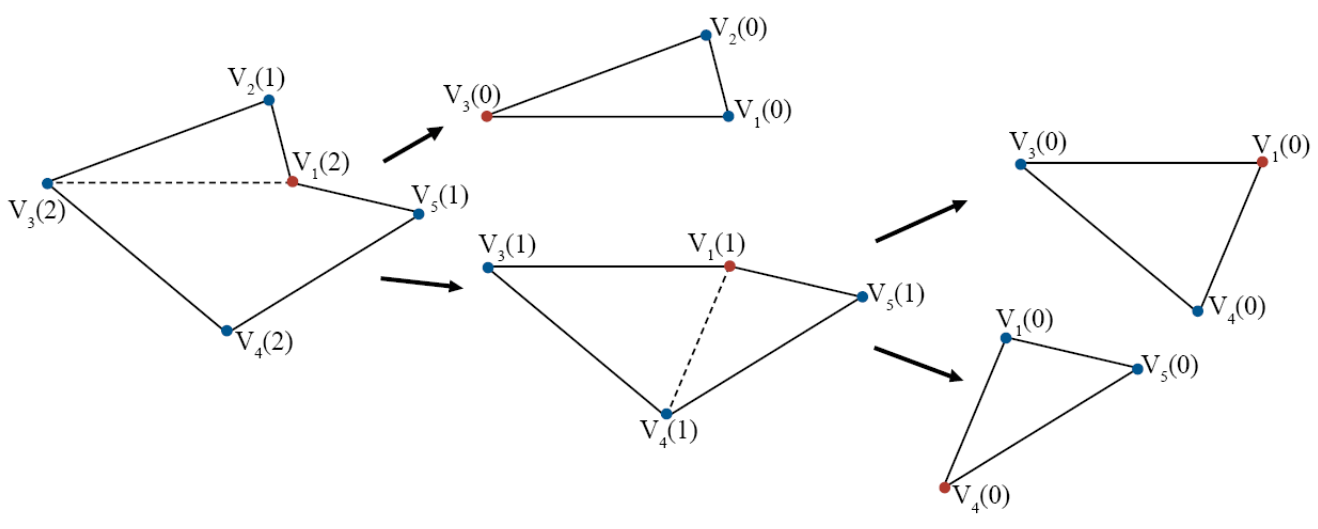
\includegraphics[width=1\textwidth]{bilder/sichtbarkeit_zerlegung.png}
    \caption[Triangulation mittels Sichtbarkeitsalgorithmus]{\centering Von links nach rechts die Schritte der Unterteilung eines Polygons in Unterpolygone bis zur Triangulierung mittels Sichtbarkeit der Eckpunkte (rot die First Heads)\cite{newAlg} }
\end{figure}
\pagebreak


\begin{table}[t]
    \begin{tabular}[h]{| c | c | c | c | c |}
    \hline
    \multicolumn{5}{|c|}{Eckenanzahl: 30 ~~~ $v_i = \left\{(x,y)| -50 < x < 50, -50 < y < 50\right\}$}\\ \hline
   Algorithmus & Polygon- & Durchschn.& Standartabw. & Durchschn. \\
   & fläche &  Dreiecksfläche & der Dreiecksfläche & min. Winkel \\ \hline
    Ear-Clipping & 4128,5px & 147,446px  & 163,63px  & 10,29° \\ \hline
    Sichtbarkeit & 4128,5px & 147,446px  & 148,91px & 15,04°\\ \hline
    \end{tabular}
    \caption[Vergleich \ac{eca} und Sichtbarkeitsalgorithmus bei rundem Polygon]{\centering Vergleich des \ac{eca} und des Sichtbarkeitsalgorithmus bei einem rundem Polygon mit 30 Ecken anhand der Standartabweichung der Dreiecksfläche in Pixeln (je kleiner desdo besser)
    und der durchschnittlichen minimalen Innenwinkelgröße in Grad (je größer desdo besser) \cite{newAlg}\linebreak\linebreak}
    \label{tab:tab2}
    
\end{table}

\begin{table}[t]
    \begin{tabular}[h]{| c | c | c | c | c |}
    \hline
    \multicolumn{5}{|c|}{Eckenanzahl: 30 ~~~ $v_i = \left\{(x,y)| -100 < x < 100, -30 < y < 30\right\}$}\\ \hline
   Algorithmus & Polygon- & Durchschn.& Standartabw. & Durchschn. \\
   & fläche &  Dreiecksfläche & der Dreiecksfläche & min. Winkel \\ \hline
    Ear-Clipping & 5066px & 180,93px & 185,50px & 9,23° \\ \hline
    Sichtbarkeit & 5066px & 180,93px & 146,03px & 16,45° \\ \hline
    \end{tabular}
    \caption[Vergleich \ac{eca} und Sichtbarkeitsalgorithmus bei länglichem Polygon]{\centering Vergleich des \ac{eca} und des Sichtbarkeitsalgorithmus bei einem länglichen Polygon mit 30 Ecken anhand der Standartabweichung der Dreiecksfläche in Pixeln (je kleiner desdo besser)
    und der durchschnittlichen minimalen Innenwinkelgröße in Grad (je größer desdo besser) \cite{newAlg}}
    \label{tab:tab3}
\end{table}
\break
\begin{flushleft}
    \vfill
\end{flushleft}





\end{onehalfspacing}

\begin{thebibliography}{11}
    \raggedright
    \bibitem{digrev}
    \emph{Digitale Revolution} \break
    (\href{https://www.staatslexikon-online.de/Lexikon/Digitale_Revolution}{https://www.staatslexikon-online.de})

    \bibitem{polynet}
    \emph{Darstellung von Kurven und Flächen}, Christoph Dähne \break
    (\href{https://www.inf.tu-dresden.de/content/institutes/smt/cg/teaching/seminars/ProseminarSS08/cdaehne/ausarbeitung.pdf}{https://www.inf.tu-dresden.de})
    
    \bibitem{sliver}
    \emph{Geometrical Mesh Quality} \break
    (\href{https://www.iue.tuwien.ac.at/phd/fleischmann/node13.html#sec:geoqual}{https://www.iue.tuwien.ac.at})

    \bibitem{sliverdef}
    \emph{Sliver In: Computer Graphics Dictionary}, Stevens, R.T., 2002.
    
    \bibitem{earclipping2}
    \emph{Triangulation by Ear Clipping}, David Eberly \break 
    (\href{https://www.geometrictools.com/Documentation/TriangulationByEarClipping.pdf}{https://www.geometrictools.com})
    
    \bibitem{polytri}
    \emph{Polygon Triangulation}, Subhash Suri \break
    (\href{https://sites.cs.ucsb.edu/~suri/cs235/Triangulation.pdf}{https://sites.cs.ucsb.edu/~suri/cs235/Triangulation.pdf}) 
    
    \bibitem{paralleleca}
    \emph{Parallelized ear clipping for the triangulation and constrained Delaunay triangulation of polygons}, Günther Eder, Martin Held, Peter Palfrader \break
    (\href{https://www.sciencedirect.com/science/article/pii/S092577211830004X}{https://www.sciencedirect.com})

    \bibitem{improvedeca}
    \emph{Improved Algoritms For Ear-CLipping Triangulation}, Bartosz Kajak, 2005 \break
    (\href{https://digitalscholarship.unlv.edu/thesesdissertations/1319/}{https://digitalscholarship.unlv.edu/thesesdissertations/1319/})

    \bibitem{newAlg}
    \emph{A comparison of Ear Clipping and a new Polygon Triangulation Algorithm}, Ran Liu \break
    (\href{https://www.diva-portal.org/smash/get/diva2:330344/FULLTEXT02.pdf}{https://www.diva-portal.org/smash/get/diva2:330344/FULLTEXT02.pdf})

    \bibitem{polydef}
    \emph{Polygon, Definition} \break
    (\href{https://mathepedia.de/Polygone.html}{https://mathepedia.de/Polygone.html})
    
    \bibitem{regpoly}
    \emph{Regular Polygons. In: Michiel Hazewinkel (Hrsg.): Encyclopedia of Mathematics. Springer-Verlag und EMS Press, Berlin 2002}
    
    \bibitem{convex}
    \emph{Convex Polygon} \break
    (\href{https://www.mathopenref.com/polygonconvex.html}{https://www.mathopenref.com/polygonconvex.html})
    
    \bibitem{polytri3}
    \emph{Triangulation, Definition} \break
    (\href{https://encyclopediaofmath.org/wiki/Triangulation}{https://encyclopediaofmath.org/wiki/Triangulation})
    
    \bibitem{simplex}
    \emph{Simplex, Definition} \break
    (\href{https://encyclopediaofmath.org/wiki/Simplex}{https://encyclopediaofmath.org/wiki/Simplex})
    
    \bibitem{earclipping}
    \emph{Ear-clipping Based Algorithms of Generating High-quality Polygon Triangulation}, Gang Mei, John C.Tipper and Nengxiong Xu \break 
    (\href{https://arxiv.org/ftp/arxiv/papers/1212/1212.6038.pdf}{https://arxiv.org/ftp/arxiv/papers/1212/1212.6038.pdf})
    
    \bibitem{polytri2}
    \emph{Ear-Clipping Triangulierung} \break
    (\href{https://wiki.delphigl.com/index.php/Ear_Clipping_Triangulierung}{wiki.delphigl.com})
   
    \bibitem{jordan}
    \emph{Jordanscher Kurvensatz} \break
    (\href{https://de.wikipedia.org/wiki/Jordanscher_Kurvensatz}{https://de.wikipedia.org})

    \bibitem{cubecut}
    \emph{The smallest 8 cubes to cover a regular tetrahedron} \break
    (\href{https://math.stackexchange.com/questions/1423014/the-smallest-8-cubes-to-cover-a-regular-tetrahedron}{https://math.stackexchange.com/})
  
    \bibitem{twoears}
    \emph{Slicing an ear using prune-and-search In: Pattern Recognition Letters}, ElGindy, H., Everett, H., and Toussaint, G. T., (1993) S. 719-722

    \bibitem{meister}
    \emph{Polygons Have Ears In: Amer. Math. Monthly}, G.H. Meisters, Ausgabe 82, S. 648–651, 1975.

    \bibitem{tm}
    \emph{Turing-Maschinen In: Der Turing Omnibus}, A. K. Dewdney, S. 211-230, 1975.

    \bibitem{orourke}
    \emph{Computational Geometry In: C. Cambridge: Cambridge University Press}, O’Rourke, J., (1998). 

    \bibitem{goodrich}
    \emph{Triangulating a polygon in parallel In: Journal of Algorithms}, M. Goodrich, Ausgabe 10, S. 327-351, 1989. \break
    (\href{https://www.sciencedirect.com/science/article/pii/0196677489900321}{https://www.sciencedirect.com/})

    \bibitem{fist}
    \emph{FIST: Fast Industrial-Strength Triangulation of Polygons In: Algorithmica}, Held, M., Ausgabe 30, S. 563–596, 2001.
    ()\href{https://link.springer.com/article/10.1007/s00453-001-0028-4}{https://link.springer.com/article/10.1007/s00453-001-0028-4})
    
    \bibitem{dnc}
    \emph{Reentrant Polygon Clipping}, Sutherland, Ivan E. und Hodgman, Gary W., 1974. \break
    (\href{https://dl.acm.org/doi/abs/10.1145/360767.360802}{https://dl.acm.org/doi/abs/10.1145/360767.360802})
\end{thebibliography}

\end{document}